%!TEX root = ../thesis.tex

%invariant environment
\newenvironment{invariants}{%
  \refstepcounter{thrm}%
  \mypar{Invariants~\theprop}%
  \renewcommand*{\theenumi}{\theprop\,(I\arabic{enumi})}%
  \renewcommand*{\labelenumi}{(I\arabic{enumi})}%
  \enumerate
}{%
  \endenumerate
}

\section{Unified Algoritmh}
\fxerror[inline]{For now this chapter assumes we did not need to make moves when creating fences}

Now we have presented sweep-line based algorithms that preserver vertical and horizontal onesidedness respectively. We will now introduce an algorithm that gives a $(k,\infty)$-sided rectangular dual for any graph without separating $4$-cycles. We will show an algorithm exists with $k=17$.


 \subsection{Fans}
 In order to effectively describe the algorithm and its proof we will have to introduce some more concepts.

 Consider a blue face $F$ in between two fences, we will call such a face a \emph{strip}. Every interior edge of this face goes from one fence to the other (due to property \ref{e:crossingEdges}). To better understand the structure of such a strip we will describe the edges from $\spl(F)$ to $\mrg(F)$ .

 Let $u_0 , u_1, \ldots u_n$ be the vertices of the upper boundary path of $F$ and $v_0, v_1, \ldots, v_m$ the vertices of the bottom boundary path. That is $u_0=v_0 = \spl(F)$ and $u_n = v_m = \mrg(F)$. Since our graph is a triangulation $u_1v_1$ must be an edge. For the second edge in the face we have two options $u_1v_2$ or $u_2v_1$, otherwise this edge and the previous one would not form a triangle. This principle holds for every subsequent edge, we can either increase a the index of the upper boundary path or the index of the bottom boundary path.\footnote{For the benefit of the readers that know this concept; Our strip is a \emph{triangle strip}.}

 We will call a maximal sequence of at least two edges increasing the index on the bottom boundary path (and thus keeping the index on the upper path fixed) a \emph{Bottom-fan} or simply \emph{B-fan} and a maximal sequence of at lest two edges increasing the index on the upper boundary path will be called a \emph{Top-fan} or just \emph{T-fan}. The \emph{size} of such a fan is the number of edges contained in the sequence. By the definition of a fan it has size of at least $2$.
 \fxnote{Or series of edges? It is not a sequence in the usual meaning.} We will simply use \emph{fans} to refer to both these \emph{types} of fans (i.e. T- and B-fans).

 We will call a fan of size $5$ or larger a \emph{large fan}. Then it is only natural that we call fans of size $2, 3$ or $4$ \emph{small fans}. This distinction may seem arbitrary but turns out to be very useful in the proof.
 \fxnote{Emphize fan in \emph{large fan} or not?}


 In a strip we alternately encounter B- and T-fans. Since if we would have two adjacent fans of the same type we would just have a single larger fan of that type.
 In Figure \ref{fig:uni:fans} we see a strip consisting of subsequently a B-fan of size $3$, a T-fan of size 2, a B-fan of size $2$, a T-fan of size $6$, a B-fan of size $3$ and a T-fan of size $3$.

 \begin{figure}[h]
   \centering
   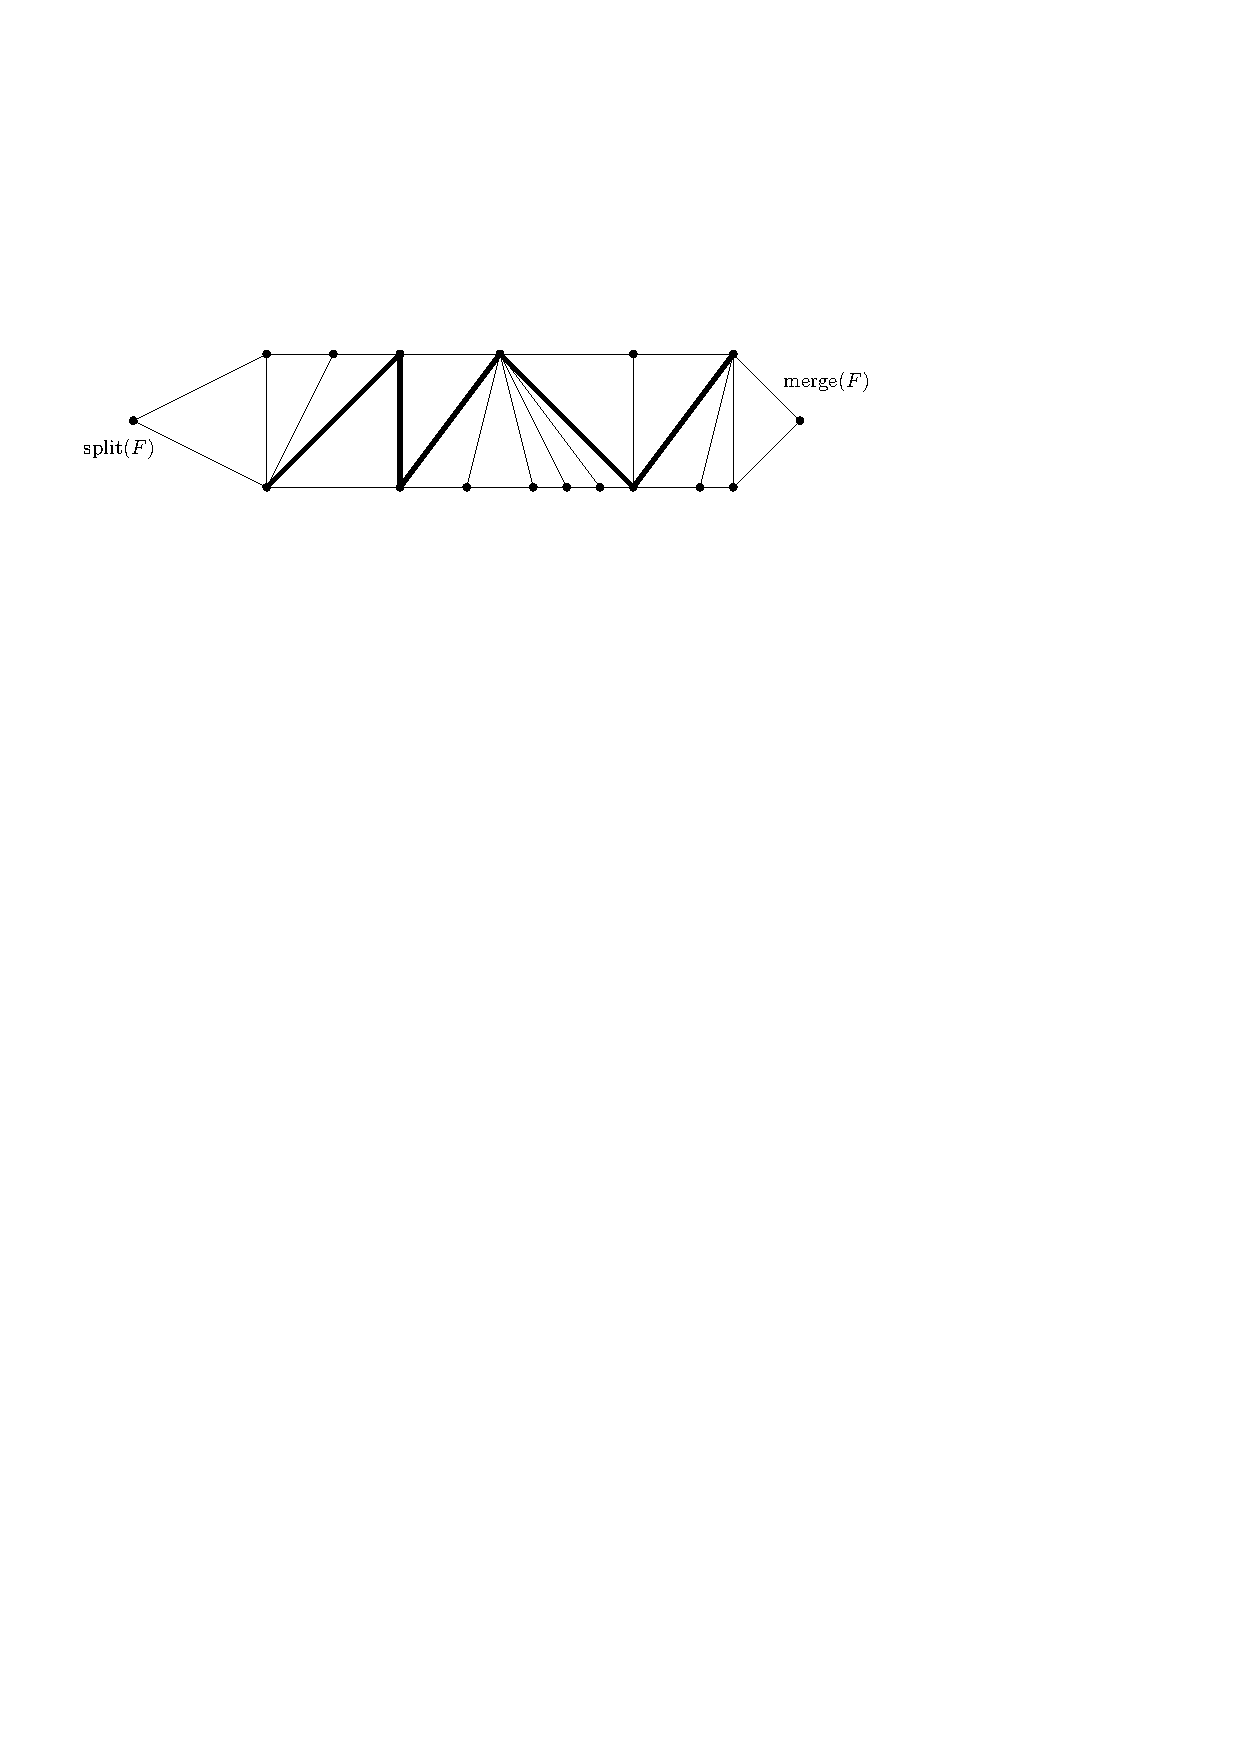
\includegraphics[scale=.9]{unifiedAlgo/img/fans}
   \caption{}
   \label{fig:uni:fans}
 \end{figure}


 We will sometimes describe a strip using a compact notation. In this notation we will denote a fan by $\text{Type}_\text{Size}$ so $B_3$ will be B-fan of size $3$ and $T_2$ a T-fan of size $2$. The strip in Figure \ref{fig:uni:fans} can be characterized by $B_2 T_2 B_2 T_5 B_3 T_3$ in this notation.

 We will expand this notation with special characters ($+,-,?, \infty$) to denote a fan without knowing it's exact size.
 We will let $T_-$ or $B_-$ imply a small fan, $T_+$ or $B_+$ a large fan, $T_?$ or $B_?$ a fan of any size and $T_\infty$ or $B_\infty$ an arbitrarily large fan.
 \footnote{this is useful in counterexamples.}




We introduce some more terminology for fans: \emph{outer edges}, \emph{fan handles} and the \emph{rim}
 \fxwarning{TODO}
\begin{figure}[h]
  \centering
  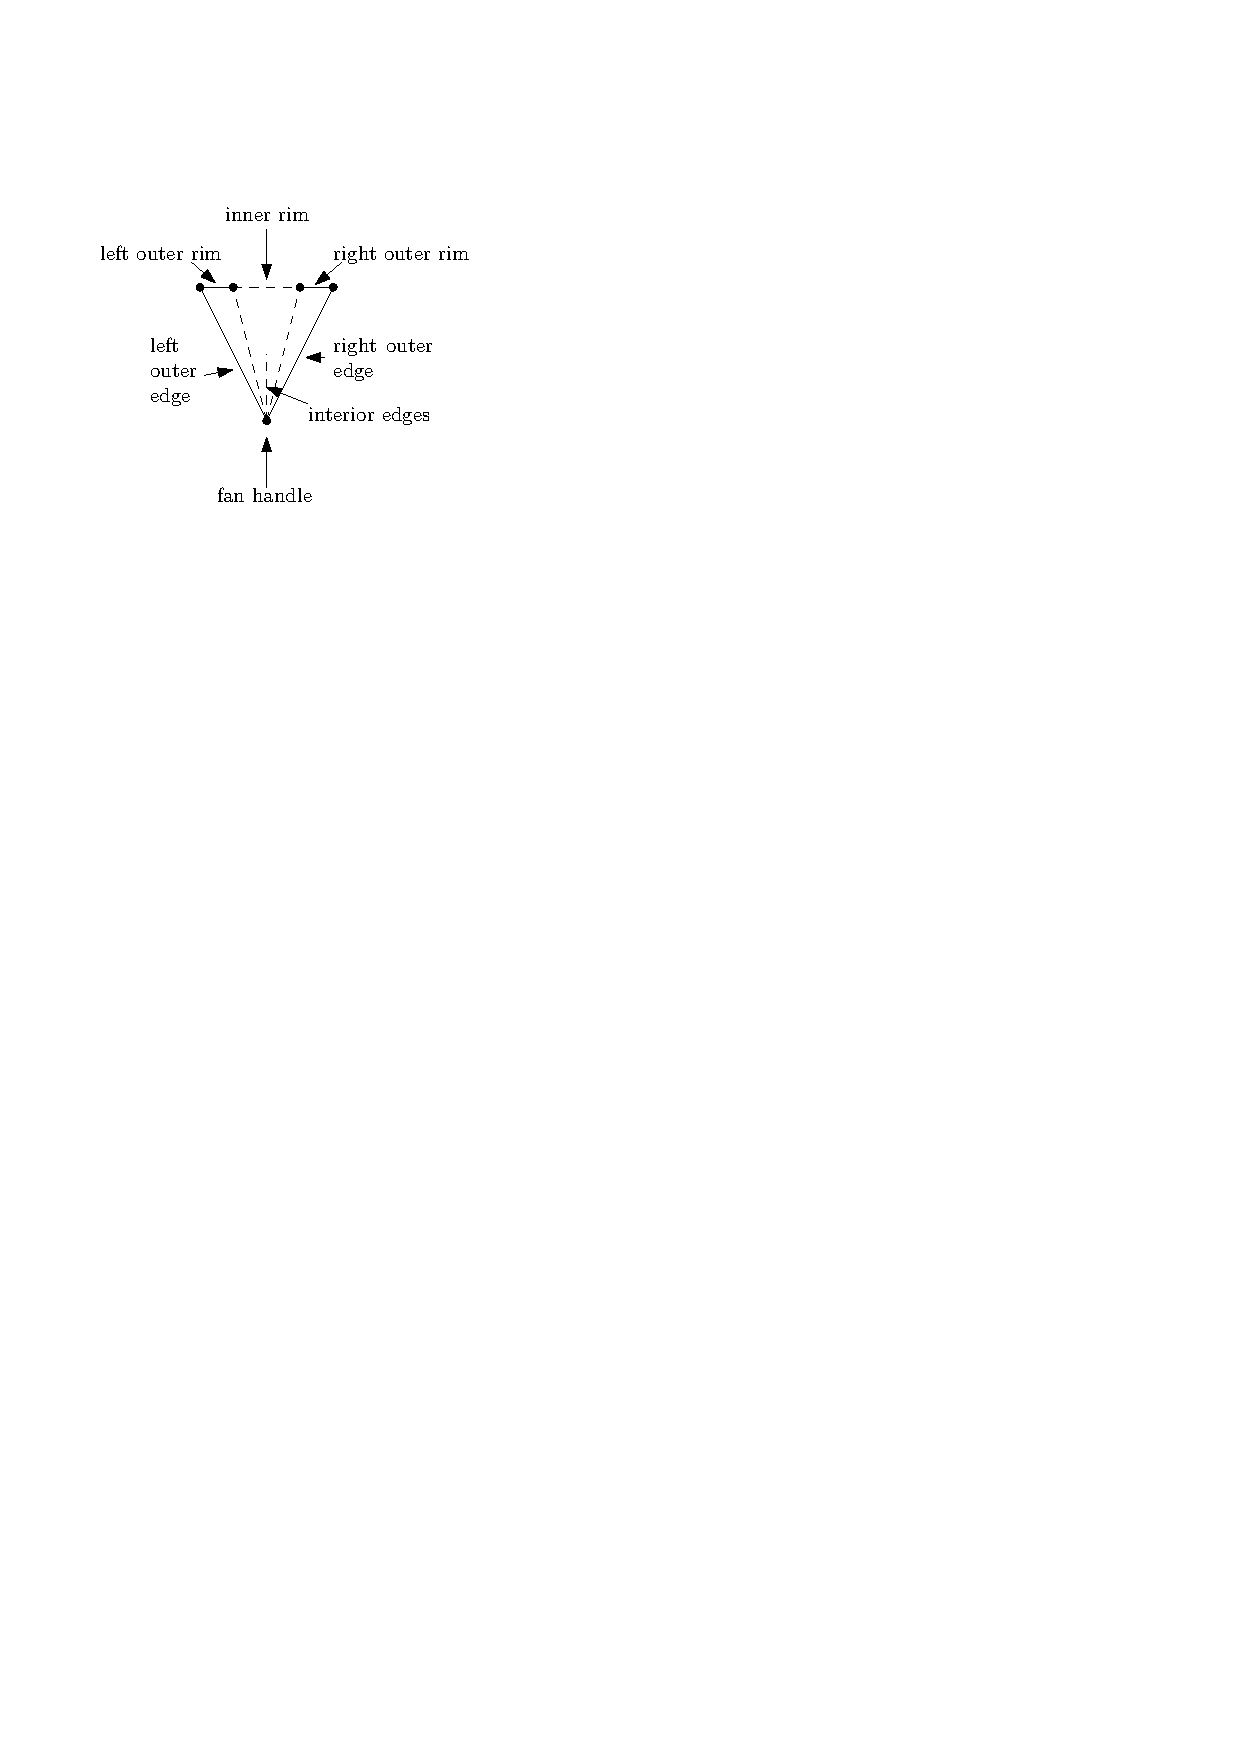
\includegraphics[scale=1]{unifiedAlgo/img/fanterms}
  \caption{}
  \label{fig:}
\end{figure}

Note that the only edges that are flippable are those that are in both a T-fan and a B-fan. This are exactly the outer edges of any fan.
\fxnote{We might want to show this}


\subsection{Blue $Z$'s and loaded edges}
  During the algorithm we will often recolor a red edge into a blue edge. When we do this we create a structure that we will refer to as a \emph{blue $Z$}. A blue $Z$ is a path of three blue edges all in the same red face with it's first and last edge on a fence.
  When we recolor a red edge in a strip into we create at least on such a blue $Z$ with it's \emph{top} and \emph{bottom} edges on the two different fences bordering this strip. Its \emph{middle} edge is the recently recolored edge.
  \fxwarning{TODO adept for moves}

  We refer to two blue $Z$'s as chained when the bottom edge of one $Z$  is the same as the top edge of the other. Chained blue $Z$'s are something we want to prevent because they indicate a large red face.
  \fxnote{explain this better?}

  In order to prevent to many blue $Z$'s from chaining we use the following technique in our algorithm. When we recolor an edge we say that the bottom edges of any blue $Z$ containing        this edge become \emph{loaded}. Any edge that is not (yet) loaded is referred to as a \emph{free} edge.
  \begin{figure}[h]
    \centering
    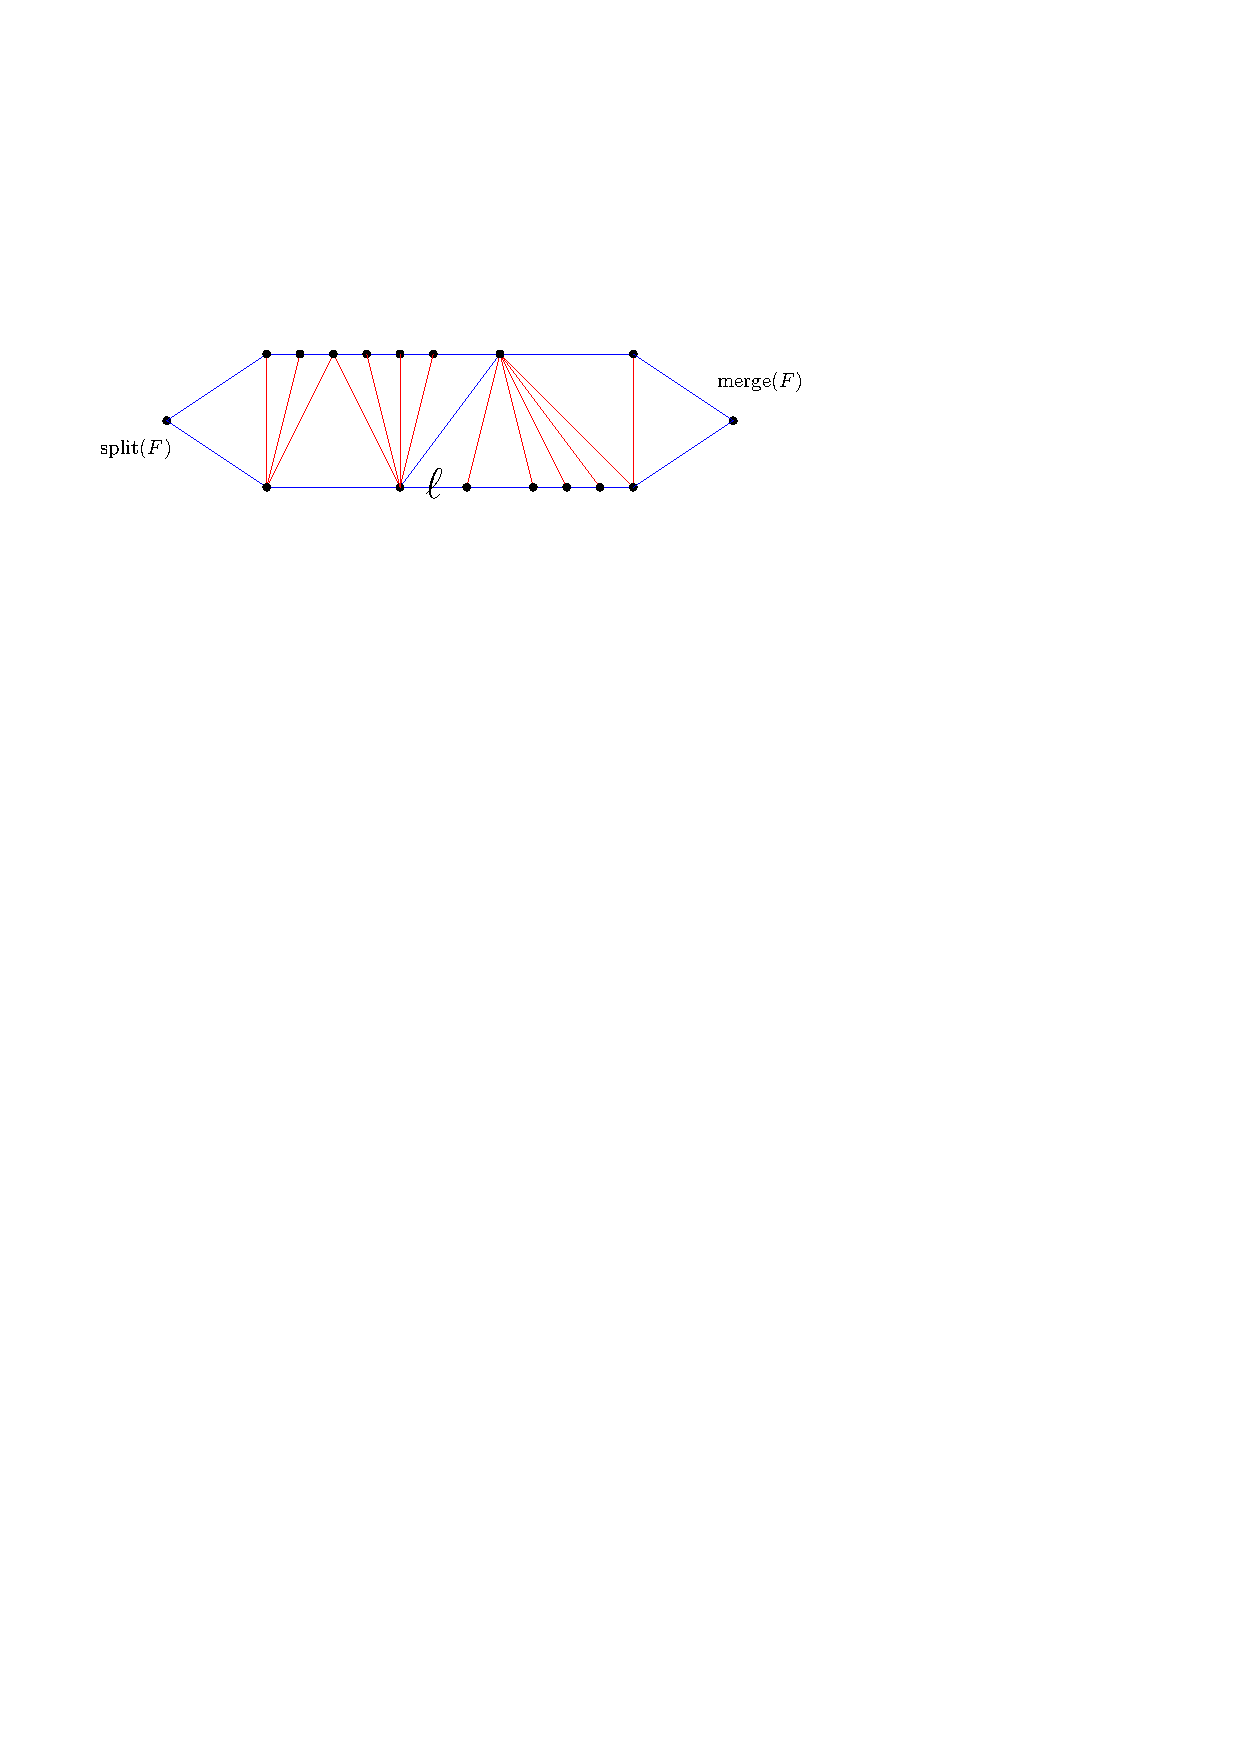
\includegraphics[scale=1]{unifiedAlgo/img/load}
    \caption{The algorithm has decided to flip an edge. The bottommost edge of the $Z$ is marked as loaded. }
    \label{fig:uni:load}
  \end{figure}


\subsubsection{Usefull lemma's}
  Before we describe the algorithm it is handy that we already show the following lemma's
  \begin{lemma}
    \label{lm:}
    A graph without overlapping blue $Z$'s is vertically $(2, \infty)$ sided.
  \end{lemma}
  This depends how we define overlap, it seems true for vertex overlap

  \begin{lemma}
    \label{lm:}
    Above B-fan we have fans of size $2$
  \end{lemma}
  \begin{proof}
    Otherwise we create a $4$-cycle
  \end{proof}


\subsection{Algorithm}

\mypar{Outline}
The approach taken by this algorithm will be the following
\begin{enumerate}
  \item Subdivided the graph by fences as in the red algorithm.
  \item We separate big B-fans from the rest of the fans in this strip
  \item If blue faces  in this strip are still too long we will flip some of their interior edges. We try to prevent the creation of new chained blue $Z$'s.
  \item We solve the blue $Z$'s we have created by doing a few flips.
\end{enumerate}

\mypar{order of strips}
There is a partial order of strips. we start with the largest element and can always treat such a strip such that all strips larger than that strip are already treated while all strips smaller than that strip are note yet treated.
 \fxwarning{TODO Does this order exists, find ref in literature}




\subsubsection{Phase 1: Finding fences}


\subsubsection{Phase 2: Removing large B-fans}

While deciding which edges to flip on each strip we will maintain the following invariants

\begin{invariants}
  \label{inv:uni:load}
  \item The edges on a fence obey the following:
  \begin{itemize}
    \item There are no more then $2$ subsequent loaded edges
    \item 1 loaded edge followed by at least 1 unloaded edge
    \item 2 loaded edges followed by at least two unloaded edges
  \end{itemize}
\end{invariants}


\begin{lemma}
  \label{lm:uni:removingLargeB-fans}
  We can create blue $(9, \infty)$-faces containing all the large B-fans while obeying Invariant \ref{inv:uni:load}.
\end{lemma}


\begin{proof}
  We will begin scanning at the split of the strip when we encounter a large B-fan ($B_+$) we  will enter a multistage case distinction ending with a small enough blue face and and edges on the bottom fence of the strip satisfying Invariant \ref{inv:uni:load}.

  Note that in all cases we flip the left outer edge of the first $B_+$ we encounter when scanning. Also note that we only ever flip edges bordering a large B-fan.


  Let us first inspect the 3 T-fans following our $B_+$. If any of them is size 5 or larger we flip the right outer edge of the last large B-fan before this T-fan and continue our scan from the fan onward. In this case the largest face we create is $(7, \infty)$.
   \fxwarning{TODO insert figure of situstion}

  Otherwise all three T-fans following our $B_+$ are small, we have the following sequence $B_+ T_- B_? T_- B_? T_- B_?$. If the rightmost B-fan is large we continue our scan at this B-fan, creating a $(9, \infty)$- face. Otherwise, if the second-right most B-fan is large we continue our scan there creating a $(6, \infty)$-face.

  Otherwise we check whether the third-rightmost B-fan is large if this is the case we flip it's \textbf{right} outer edge and continue our scan after this B-fan. Otherwise we also flip the \textbf{right} outer edge of the original $B_+$. We continue the scan right after this flipped edge. In both cases we can do this without offending Invariant \ref{inv:uni:load} since the next two/three B-fans are small so the next one/two edges will not be loaded even when continuing the scan immediately after. These last two steps yield faces of size at most $(4, \infty)$.

  One can also see the order in which we try to place edges in Figure \ref{fig:uni:placeedges}

  \begin{figure}[h]
    \centering
    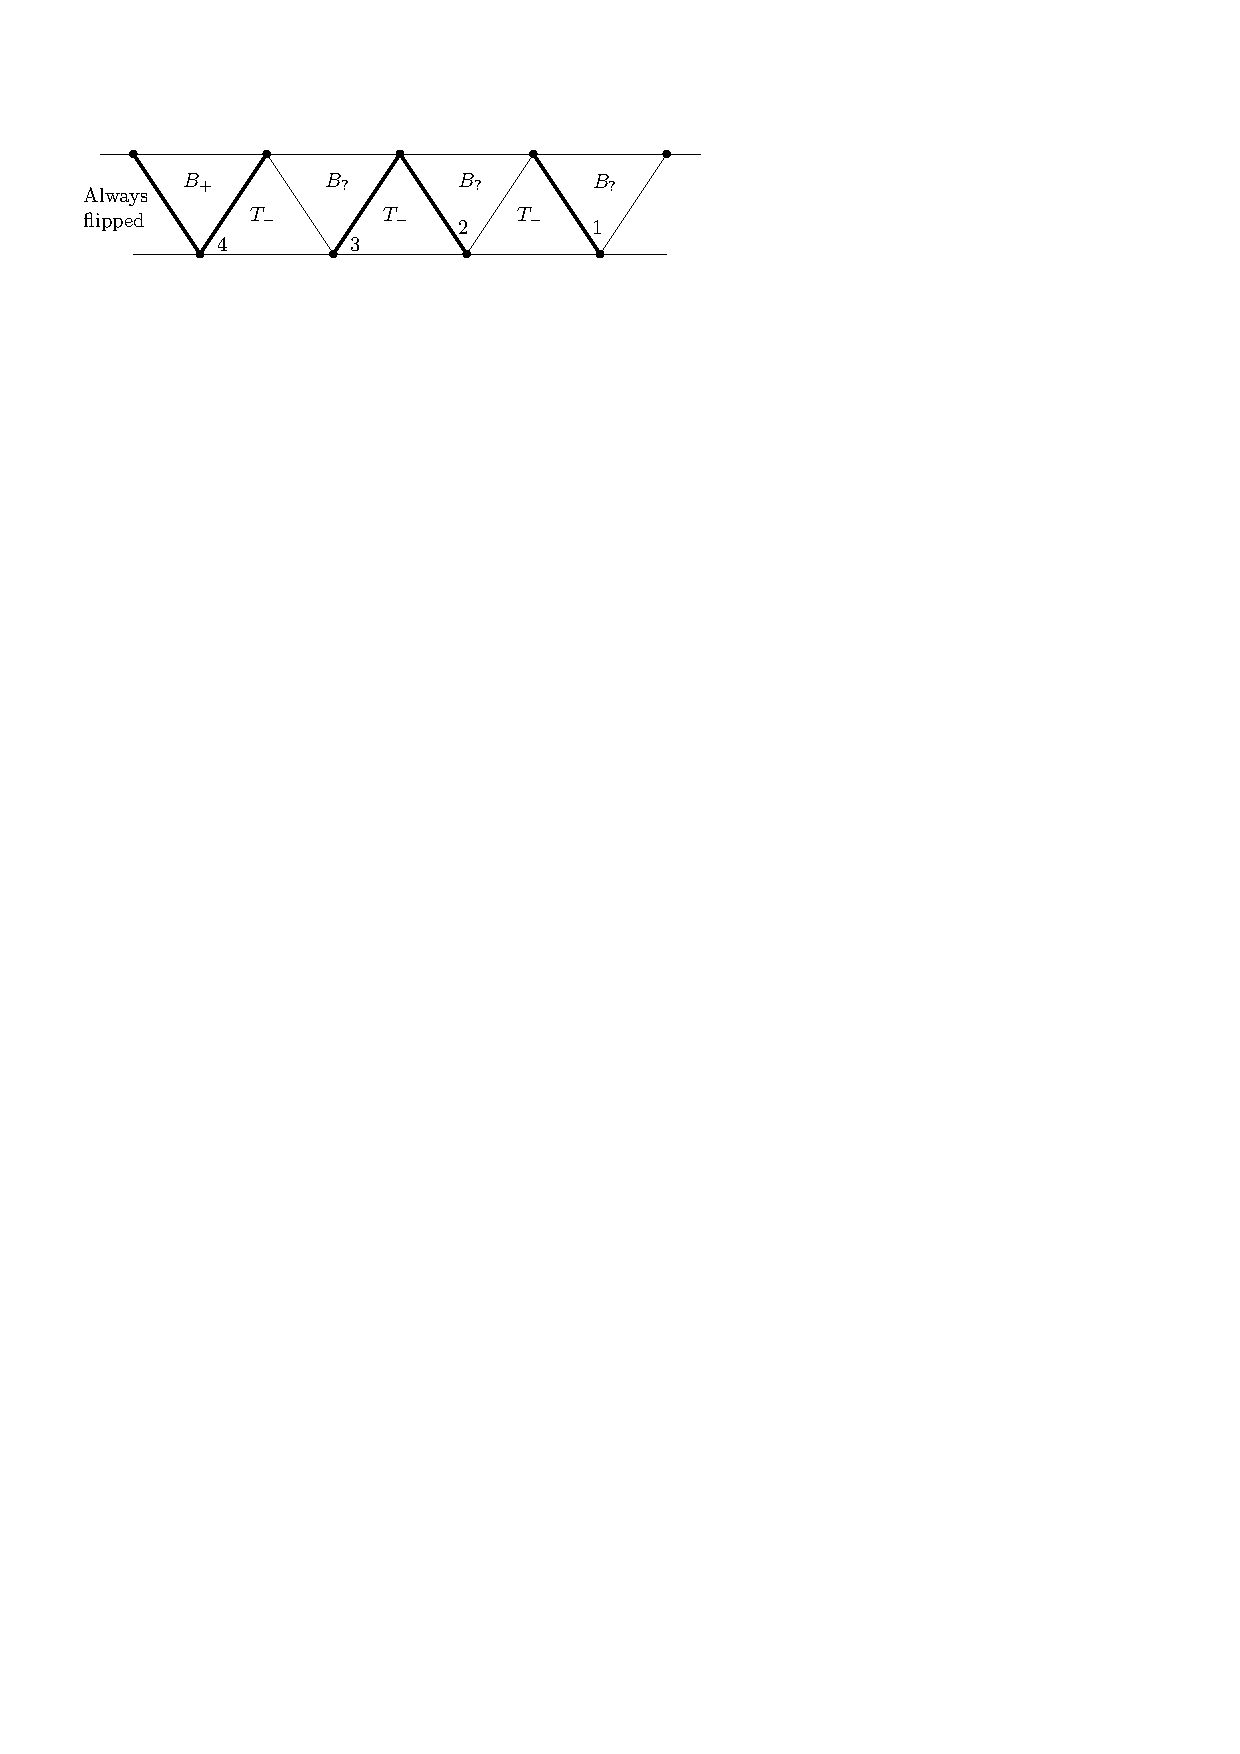
\includegraphics[scale=1]{unifiedAlgo/img/placeEdges}
    \caption{Order in which we try to flip edges. We only flip an edge if it neighbors a large B-fan.}
    \label{fig:uni:placeedges}
  \end{figure}

  Trough this case distinction we've seen that we indeed can create blue $(9,\infty)$-faces containing all the large B-fans while obeying Invariant \ref{inv:uni:load}.

\end{proof}

  Note that we only ever flipped outer edges of a $B_+$ in this proof


\subsubsection{Phase 3: The rest of the strip}
Any further blue faces that are still to large do not contain any large B-fans. We will be careful to flip only if we satisfy the following invariants in addition to Invariants \ref{inv:uni:load}

\begin{invariants}
  \label{inv:uni:rest}
  \item We do not flip an edge creating a blue $Z$ containing a loaded edge.
  \label{inv:uni:noLoad}
  \item We do not flip an edge creating a blue $Z$ containing a pad of a large B-fan in the next
   strip.
  \label{inv:uni:noPad}
\end{invariants}

 \fxwarning{TODO give these a proper ref and environment (beore starting real proofs)}

We consider two cases for our still to large blue face $F$, either this blue face is above the entirety of a large B-fan in the next strip or it isn't.
In the first case we can find a flippable edge satisfying all the invariants and we are done.

\begin{lemma}
  \label{lm:uni:flipAboveLargeB-fan}
  We can flip at least one edge above in any blue face that lies above the entirety of a large B-fan in the next strip.
  \fxnote{This lemma should probably change when we start to allow moves}
\end{lemma}
\begin{proof}
  In the strip above a large B-fan and directly above such a large B-fan any T-fan can only be of size $2$ since otherwise we would have a separating $4$-cycle \fxnote{I could/should make this a lemma somewhere}. Furthermore there can not be large B-fan in the face we are treating since all large B-fans are in $(9,\infty)$ faces.  We are thus in the situation depicted in Figure \ref{fig:uni:flipAboveLargeB-fan}.

  \begin{figure}[h]
    \centering
    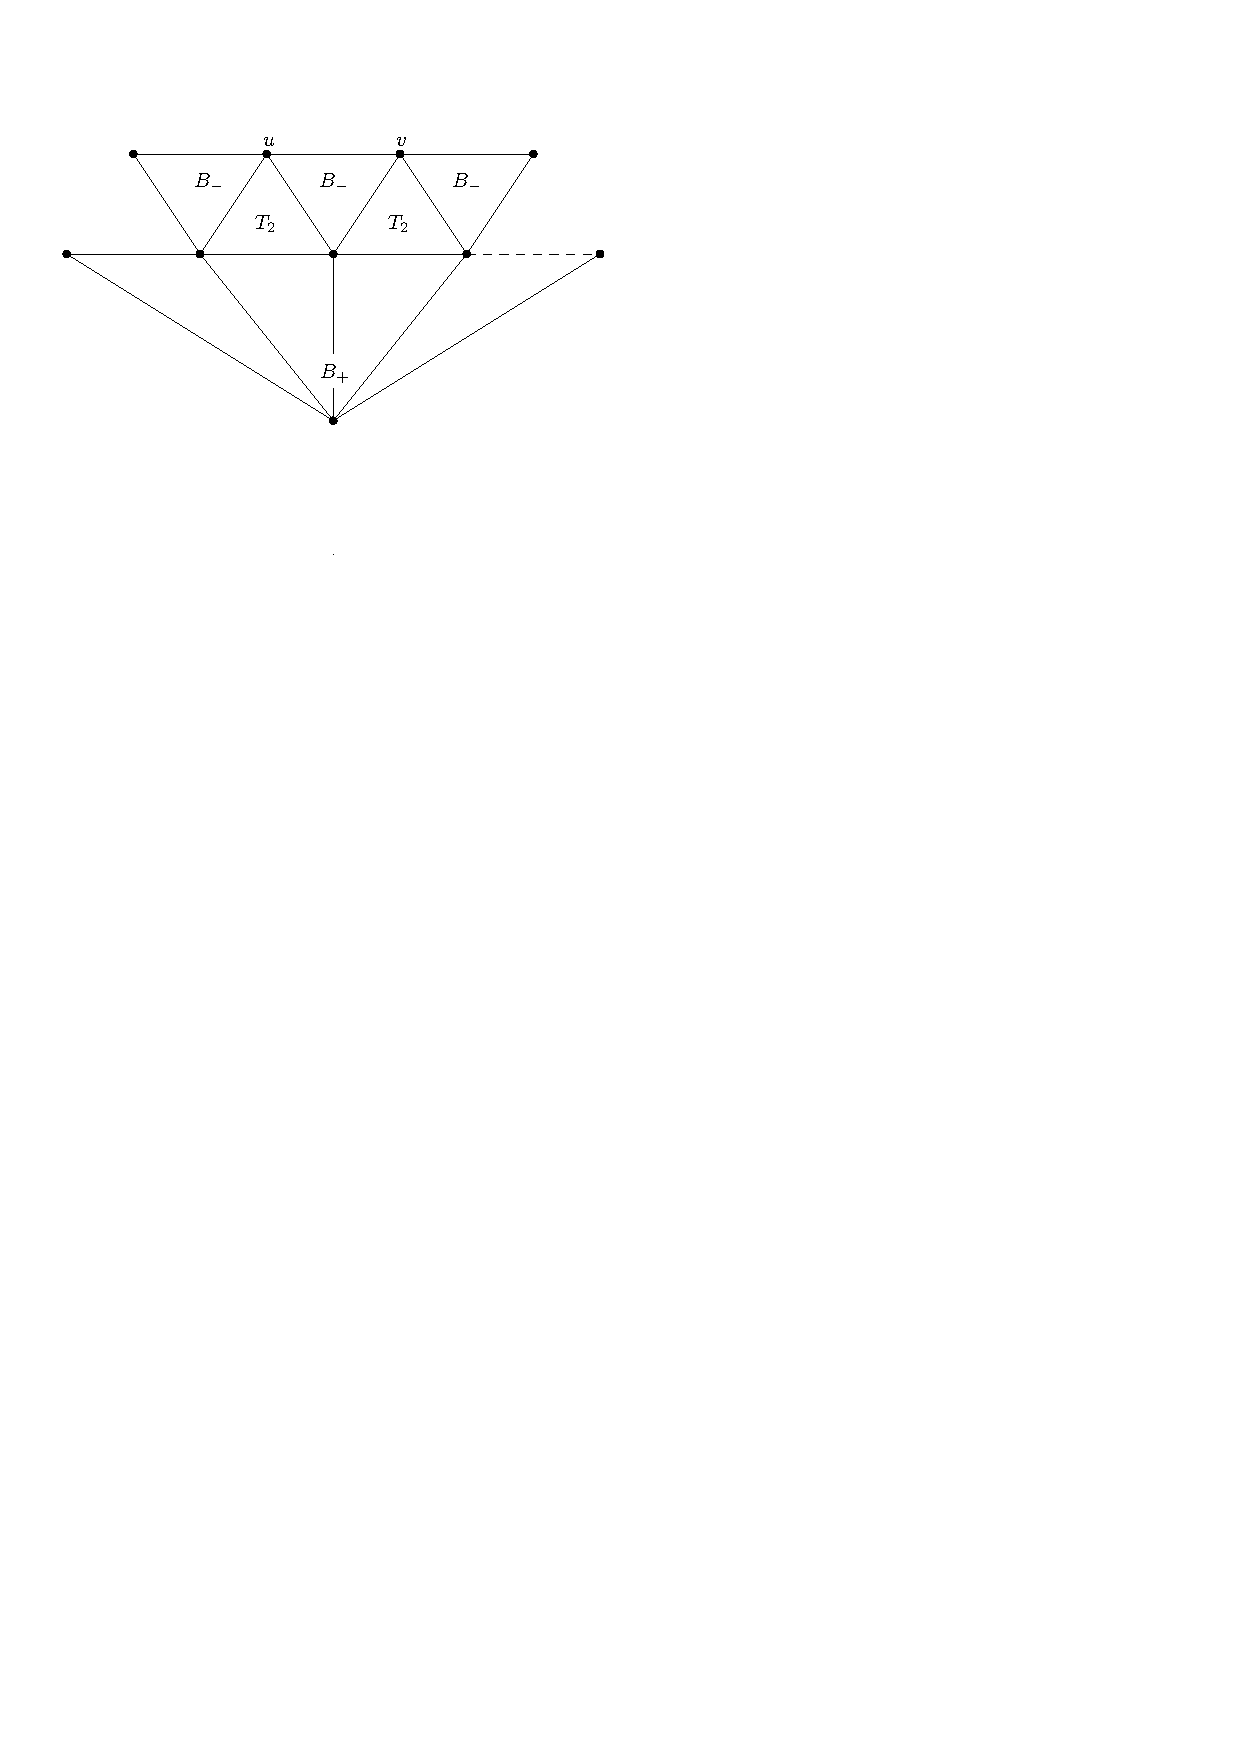
\includegraphics[scale=1]{unifiedAlgo/img/flipAboveLargeBfan}
    \caption{}
    \label{fig:uni:flipAboveLargeB-fan}
  \end{figure}

  Now suppose one of the edges neighboring $u$ is not loaded then we can flip here. Now let us assume both edges incident to $u$ on the fence are loaded then at least one of the edges of the fence incident to $v$ is unloadned  because the next two edges are unloaded due to Invariant \ref{inv:uni:load}.

  Hence we can alway flip an edge above a large B-fan.
\end{proof}


In the second case we do not have to consider more then one right pad and more the one left pad otherwise we could execute Lemma \ref{lm:uni:flipAboveLargeB-fan}

\begin{lemma}
  \label{lm:}
  In any blue face that is not a $(31, \infty)$ blue face  we can flip a edge.
\end{lemma}
\begin{proof}
  The face under consideration does not lie above the enirty of any B-fan becuase of Lemma \ref{lm:uni:flipAboveLargeB-fan}.
   \fxwarning{TODO fix this on right side only need one edge of seperation}

  Such a face that is not $(31, \infty)$ has at least $32$ vertices on the top fence. This means it has at least $31$ edges lying in at least $11$ B-fans. These B-fans have $10$ inbetween T-fans. The two T-fans  closest to the both border of the face will remain unloaded in order to preserve Invariant \ref{inv:uni:load}. This leaves $6$ fans. One pad or two loaded edges can possibly block an entire T-fan. We can not block two subsequent T-fans with loaded edges due to the fact that only small B-fans. We only have two pads. So one of the fans has to remain free and we can thus flip an edge satisfying both Invariants \ref{inv:uni:load} and \ref{inv:uni:rest}.
\end{proof}


\subsubsection{Phase 4: Flips}
After we have treated all strips the only chained blue $Z$'s are those that have their middle edge (the one crossing a strip) as outer edge of a large B-fan. This because the rest of the edges has been placed obeying the properties above.

We then have essentially two cases which occur around  both the left and right outer rim of the large B-fan. Giving us a total of at most $4$ flip operations above a large B-fan.
 \fxwarning{TODO argue this}

They are depicted in Figures \ref{fig:uni:flipcasea} and \ref{fig:uni:flipcaseb}  and we treat these as depicted in Figures \ref{fig:uni:flipactiona} and \ref{fig:uni:flipactionb}.


\begin{figure}[h]
  \centering
  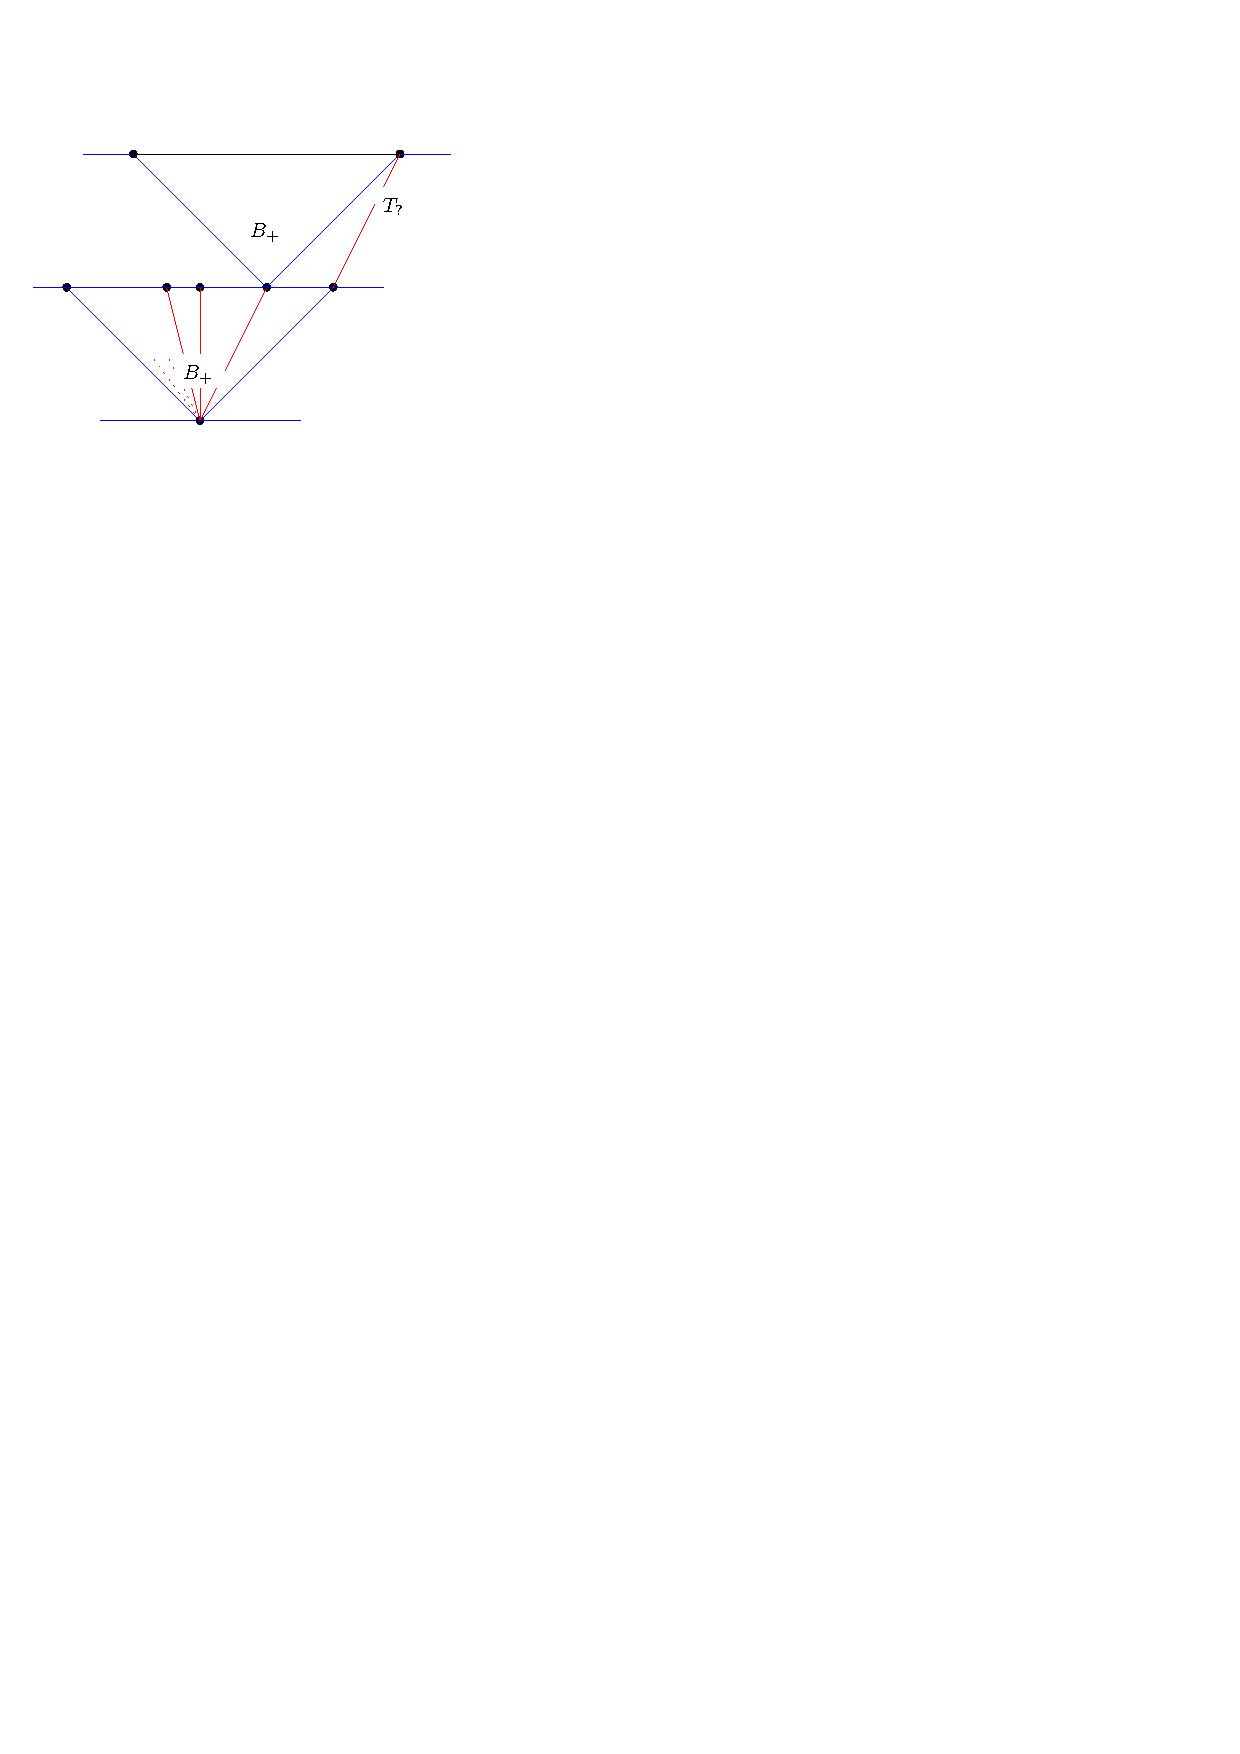
\includegraphics[scale=1]{unifiedAlgo/img/flipcasea}
  \caption{Case a) before the flip}
  \label{fig:uni:flipcasea}
\end{figure}

\begin{figure}[h]
  \centering
  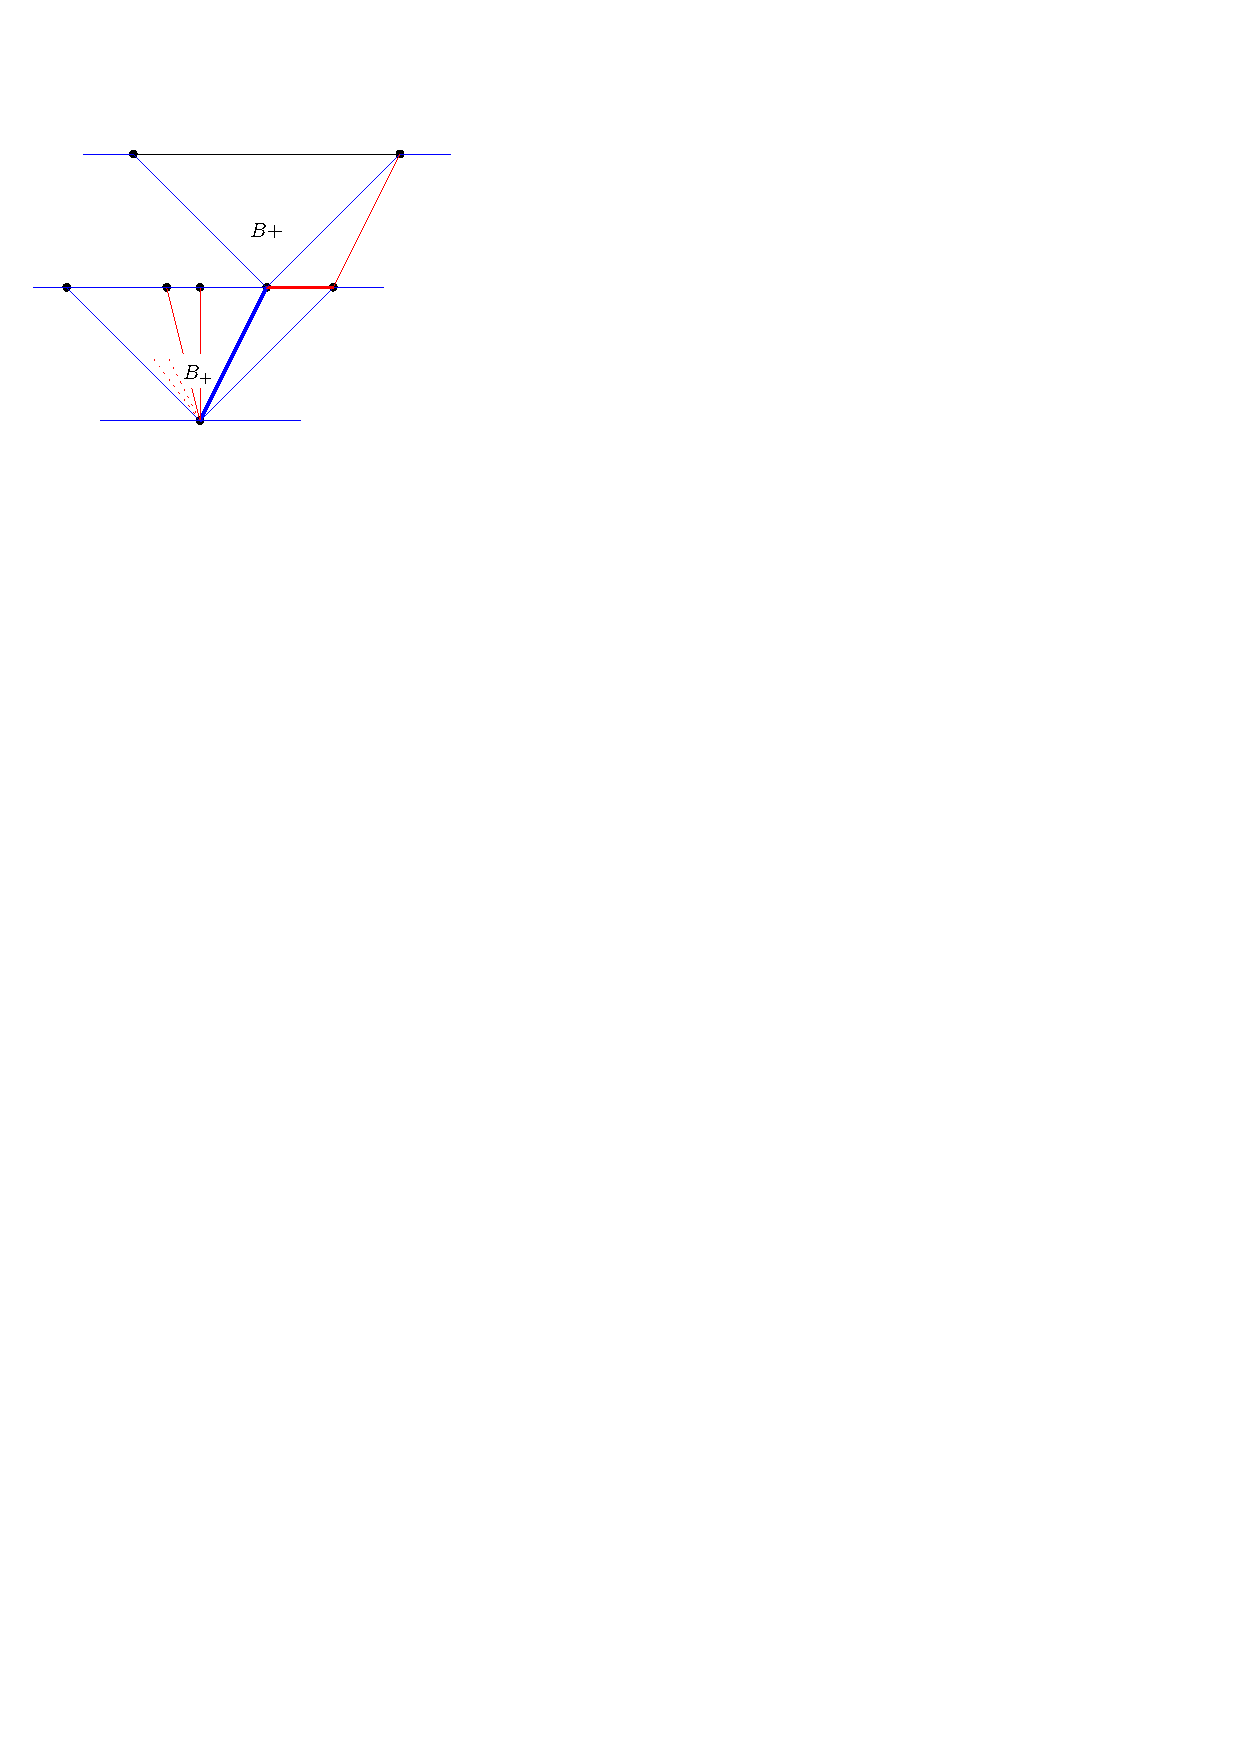
\includegraphics[scale=1]{unifiedAlgo/img/flipactiona}
  \caption{Case a) after the flip}
  \label{fig:uni:flipactiona}
\end{figure}

\begin{figure}[h]
  \centering
  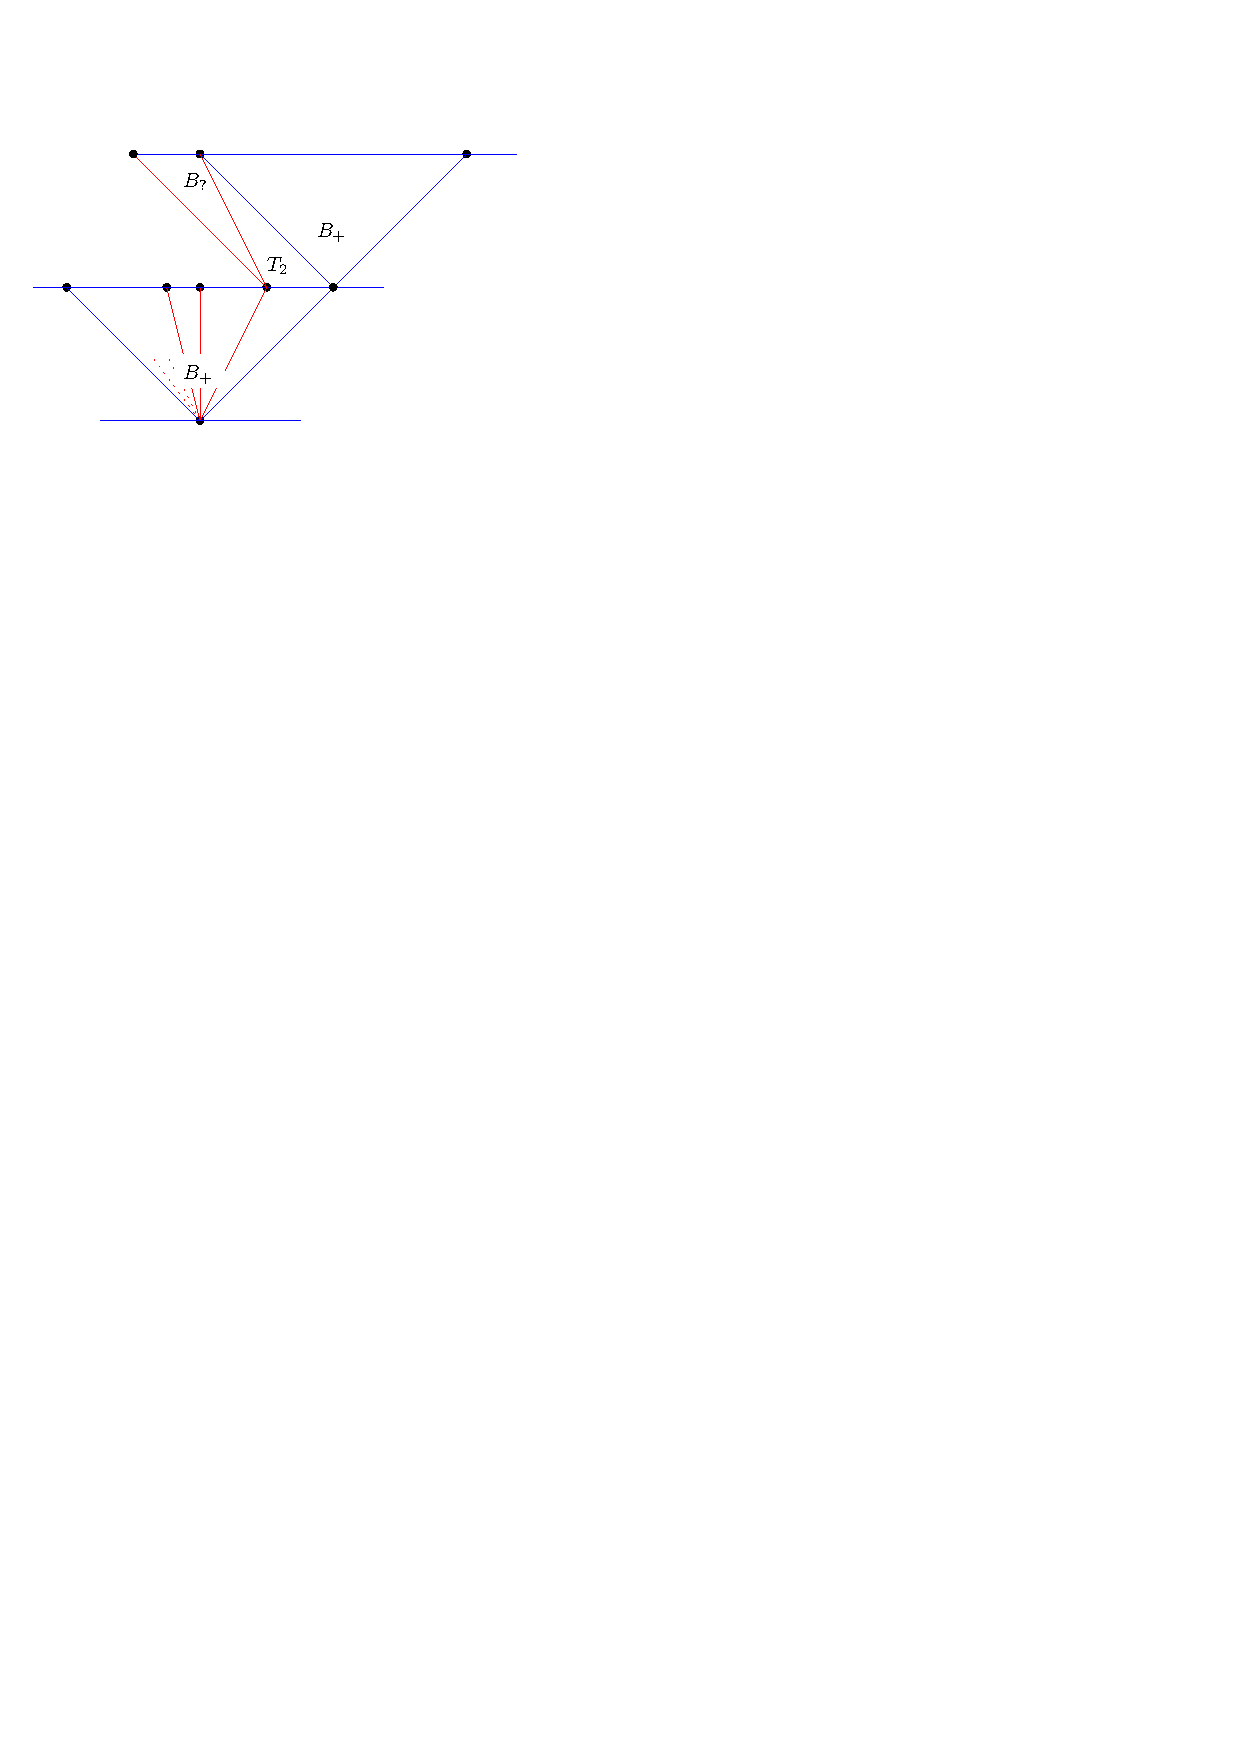
\includegraphics[scale=1]{unifiedAlgo/img/flipcaseb}
  \caption{Case b) before the flip}
  \label{fig:uni:flipcaseb}
\end{figure}

\begin{figure}[h]
  \centering
  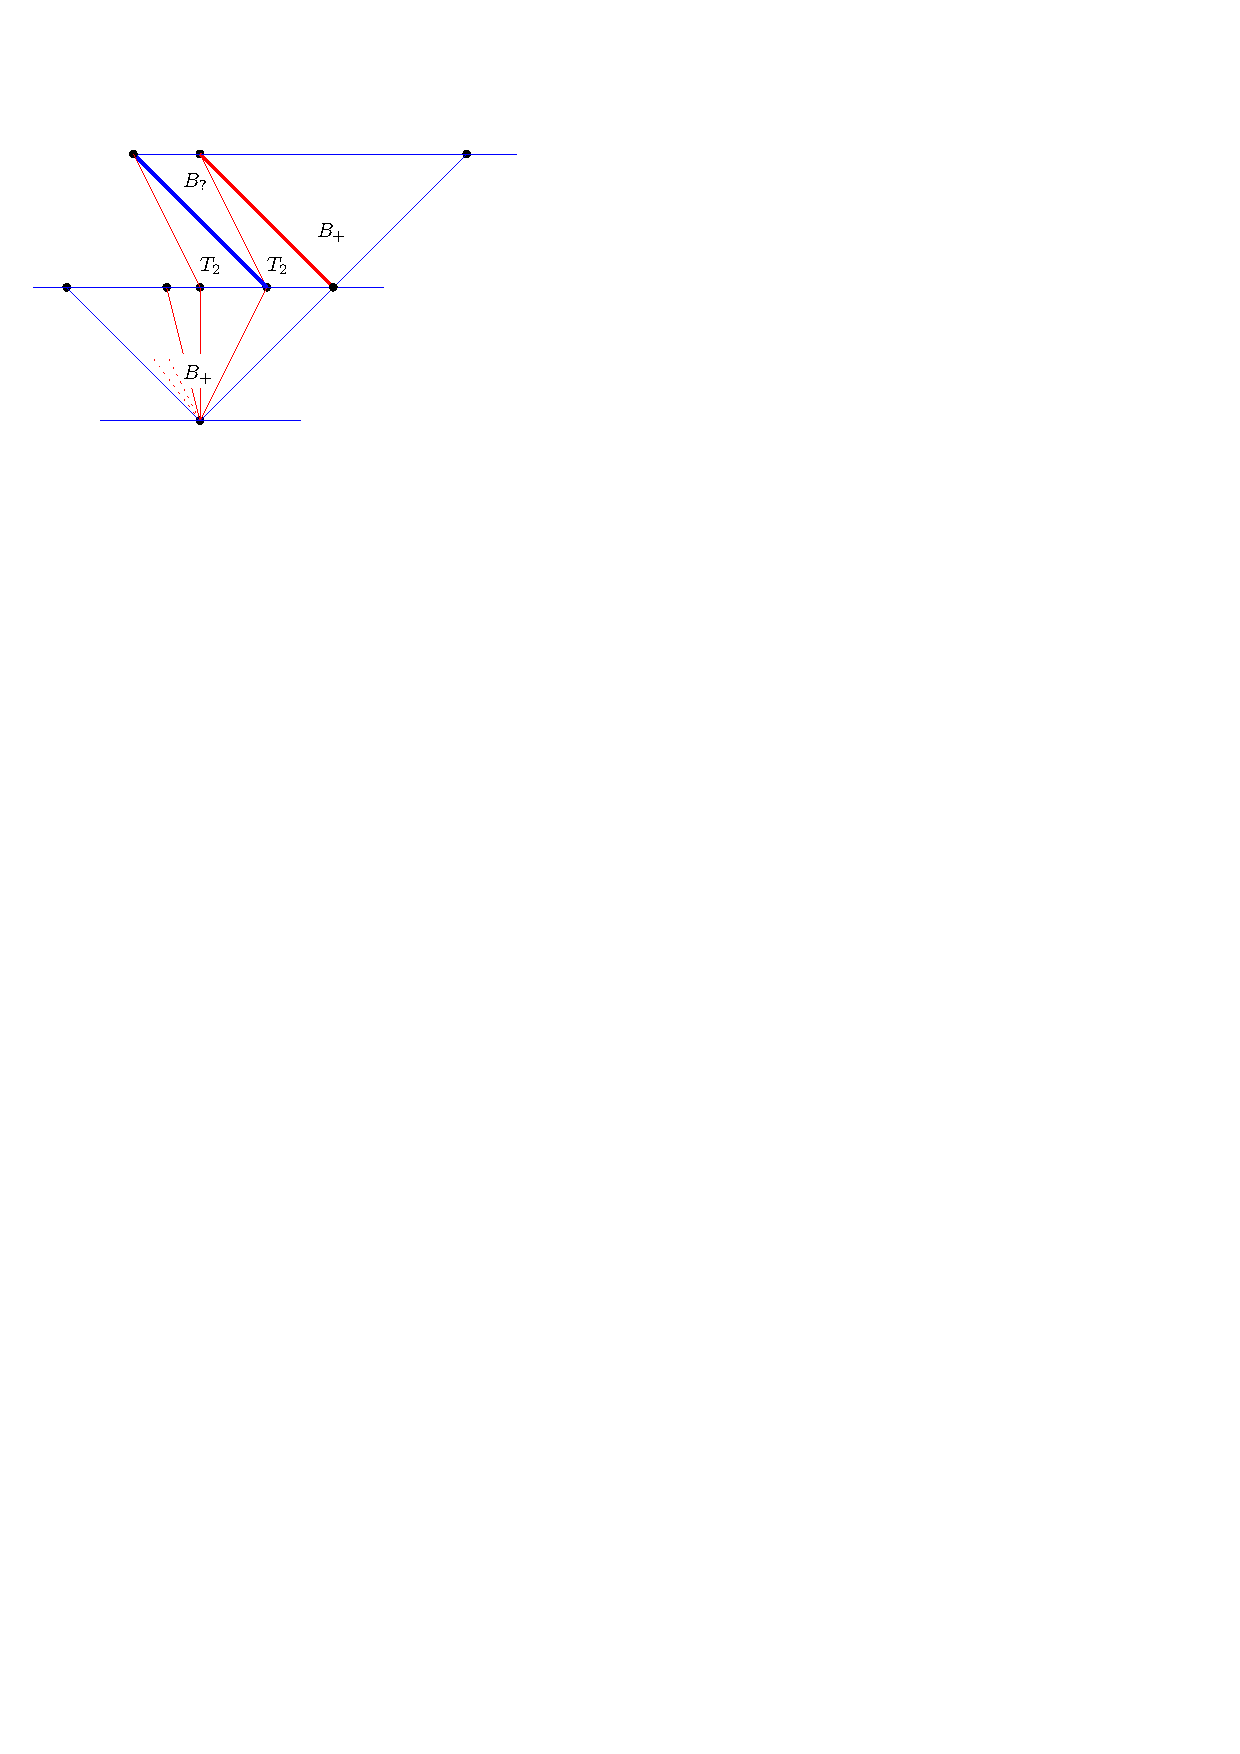
\includegraphics[scale=1]{unifiedAlgo/img/flipactionb}
  \caption{Case b) after the flip}
  \label{fig:uni:flipactionb}
\end{figure}

We will now also describe how each flip is executed and that each flip individually maintains a \rel.

\mypar{Flip type a)}
\fxwarning{TODO}

\mypar{Flip type b)}
\fxwarning{TODO}




It can be that a flip of case a) necessitates doing a flip of type b). However then we are done.

Above a B-fan of size $5$ or $6$ we would not produces a legal \rel if we do all $4$ flips. Since the B-fan would become only size $3$ after the two $a)$ flips and we need a B-fan of size $5$ to do both $b)$ flips without them interfering.

Lucky enough for us this is not a problem as the Algorithm proposed in Lemma \ref{lm:uni:removingLargeB-fans} does only color all $4$ edges necessitating a flip blue above B-fans of size $7$ or more which we will show in Lemma below.



\begin{lemma}
  \label{lm:uni:flips}
  Doing these flips we remove all chained blue $Z$'s in a finite amount of flips
\end{lemma}

\begin{proof}
  \begin{enumerate}
    \item Every chain of $Z$'s only occurs if both middle edges are adjacent to a large B-fan.
    \item We can break such a chain in the second $Z$ for every chain doing only at most 4 flips for every large B-fan.
    \item Doing any or all of these flips on a B-fan of size $7$ or more yields a valid \rel
    \item On a B-fan of size $5$ or $6$ at most three flips are available and necessary. We can do any or all of them and yield a valid \rel
    \item After doing all available flips for a B-fan there is no longer any chain of blue $Z$'s using the edges of that B-fan.
    \item Doing these flips only increases the length of any face by $2$. (what is the length of a face)
  \end{enumerate}

  \mypar{Every chain of $Z$'s only occurs if both middle edges are adjacent to a large B-fan}
  A chain of $Z$'s can only start if a first $Z$ is followed by a second $Z$. By Invariant \ref{inv:uni:noLoad} this can only happen when placing edges around a large B-fan. The middle edge of the second $Z$ is thus adjacent to a large B-fan. The middle edge of the first $Z$ is also adjacent to large B-fan since it also can not have been placed in the second phase of the algorithm due to Invariant \ref{inv:uni:noPad}.

  \mypar{We can break such a chain in the second $Z$ for every chain doing only at most 4 flips for every large B-fan}
  Given any chain of blue $Z$'s we will try to do a flip in the disrupt the chain. Given any large B-fan there are at most two edges of this B-fan colored blue (the outer edges). Only these two edges can be middle edges for some blue $Z$. The edges on the strip above this B-fan can only be above this $Z$ in one way (either type a) or b) ) without creating a monocolored triangle (which is forbidden). However doing a flip of type a) may then necessitate a flip of type b).
  \fxnote{Figure?}

  Hence we might need $4$ flips in total.

  \mypar{Doing any or all of these flips on a B-fan of size $7$ or more yields a valid \rel}
  It is clear that every flip on it's own changes a valid \rel into another valid \rel.
  When we inspect the descriptions of the flips we see that they do not interfere with each other.
  \fxnote{Expand ?}

  \mypar{On a B-fan of size $5$ or $6$ at most three flips are available and necessary. We can do any or all of them and yield a valid \rel}
  Suppose we force these $4$ flips to happen on B-fan of size $5$ or $6$ then the fence above this B-fan offends Invariant \ref{inv:uni:load}
  \fxnote{Figure?}


  \mypar{After doing all available flips for a B-fan there is no longer any chain of blue $Z$'s using the edges of that B-fan.}
  It is clear that each flip break the original chain
  Argue that flips do not introduce (too long) chains

  \mypar{Doing these flips only increases the length of any face by $2$.}
  It is clear every flip only increase face length with $1$.
  \fxwarning{TODO Make this precise for red/blue faces}

  Argue that every face is in at most $2$ flips.



\end{proof}

\fxnote{I feel the order of treatment of strips is important and i've not yet used it.}

Then after doing these flips we do not have any subsequent blue $Z$'s Except for after a flip of type b) While we sometimes have enlarged faces with $1$.  Hence the final coloring has $(3, \infty)$ red faces and $(33, \infty)$ blue faces.
